\section{Results and Analysis} \label{Sec: Result}

We present the results of our obsevation for the eight classifiers as the Table \ref{tab: observed result}.
Overall, we can achieve closely to the results as proposed by Ilhan et al \cite{kilincer2021machine}.
We present the results of comparison between our implementation and the proposed results in Figure \ref{fig: comparison}.

Overall, the accuracy scores of our implemented models are close to those of proposed results.
However, our precision, recall, geometricall mean and f1 are mostly higher.
The best score for intrusion detection as proposed by Ilhan et al. \cite{kilincer2021machine} was 99.46\% for SVM Cubic, 99.64\% for KNN fine and 99.92\% for fine tree.
While our SVM Cubic score lower at 98.27\%, KNN fine and fine tree was comparatively at 99.73\% and 99.64\%.

Interestingly, in our own solutions, the score for accuracy, precision, recall and f1 are equal, that means the number of false positive prediction is equal to false negative.
While adaptive boost model has overall lower score, our voting model can reach the range of 99\%.


\begin{table}
    \begin{tabular}{llrrrrr}
        \toprule
        model         & result & accuracy & precision & recall   & geo mean & f1       \\
        \midrule
        SVM Linear    & best   & 0.981826 & 0.981826  & 0.981826 & 0.988618 & 0.981826 \\
                      & mean   & 0.971675 & 0.971675  & 0.971675 & 0.982234 & 0.971675 \\
                      & std    & 0.003544 & 0.003544  & 0.003544 & 0.002228 & 0.003544 \\
        SVM Quadratic & best   & 0.978280 & 0.978280  & 0.978280 & 0.986391 & 0.978280 \\
                      & mean   & 0.969557 & 0.969557  & 0.969557 & 0.980906 & 0.969557 \\
                      & std    & 0.003411 & 0.003411  & 0.003411 & 0.002147 & 0.003411 \\
        SVM Cubic     & best   & 0.982270 & 0.982270  & 0.982270 & 0.988896 & 0.982270 \\
                      & mean   & 0.971948 & 0.971948  & 0.971948 & 0.982408 & 0.971948 \\
                      & std    & 0.003395 & 0.003395  & 0.003395 & 0.002138 & 0.003395 \\
        KNN Fine      & best   & 0.996897 & 0.996897  & 0.996897 & 0.998060 & 0.996897 \\
                      & mean   & 0.992173 & 0.992173  & 0.992173 & 0.995104 & 0.992173 \\
                      & std    & 0.001782 & 0.001782  & 0.001782 & 0.001116 & 0.001782 \\
        KNN Medium    & best   & 0.992908 & 0.992908  & 0.992908 & 0.995564 & 0.992908 \\
                      & mean   & 0.983041 & 0.983041  & 0.983041 & 0.989374 & 0.983041 \\
                      & std    & 0.002766 & 0.002766  & 0.002766 & 0.001734 & 0.002766 \\
        KNN Cubic     & best   & 0.994238 & 0.994238  & 0.994238 & 0.996396 & 0.994238 \\
                      & mean   & 0.987720 & 0.987720  & 0.987720 & 0.992313 & 0.987720 \\
                      & std    & 0.002246 & 0.002246  & 0.002246 & 0.001408 & 0.002246 \\
        Tree Fine     & best   & 0.983156 & 0.983156  & 0.983156 & 0.989452 & 0.983156 \\
                      & mean   & 0.966288 & 0.966288  & 0.966288 & 0.978844 & 0.966288 \\
                      & std    & 0.003827 & 0.003827  & 0.003827 & 0.002406 & 0.003827 \\
        Tree Medium   & best   & 0.998670 & 0.998670  & 0.998670 & 0.999169 & 0.998670 \\
                      & mean   & 0.993561 & 0.993561  & 0.993561 & 0.995972 & 0.993561 \\
                      & std    & 0.001847 & 0.001847  & 0.001847 & 0.001156 & 0.001847 \\
        \bottomrule
    \end{tabular}
    \caption{The results observed from different classifiers.}
    \label{tab: observed result}
\end{table}

\begin{figure}
    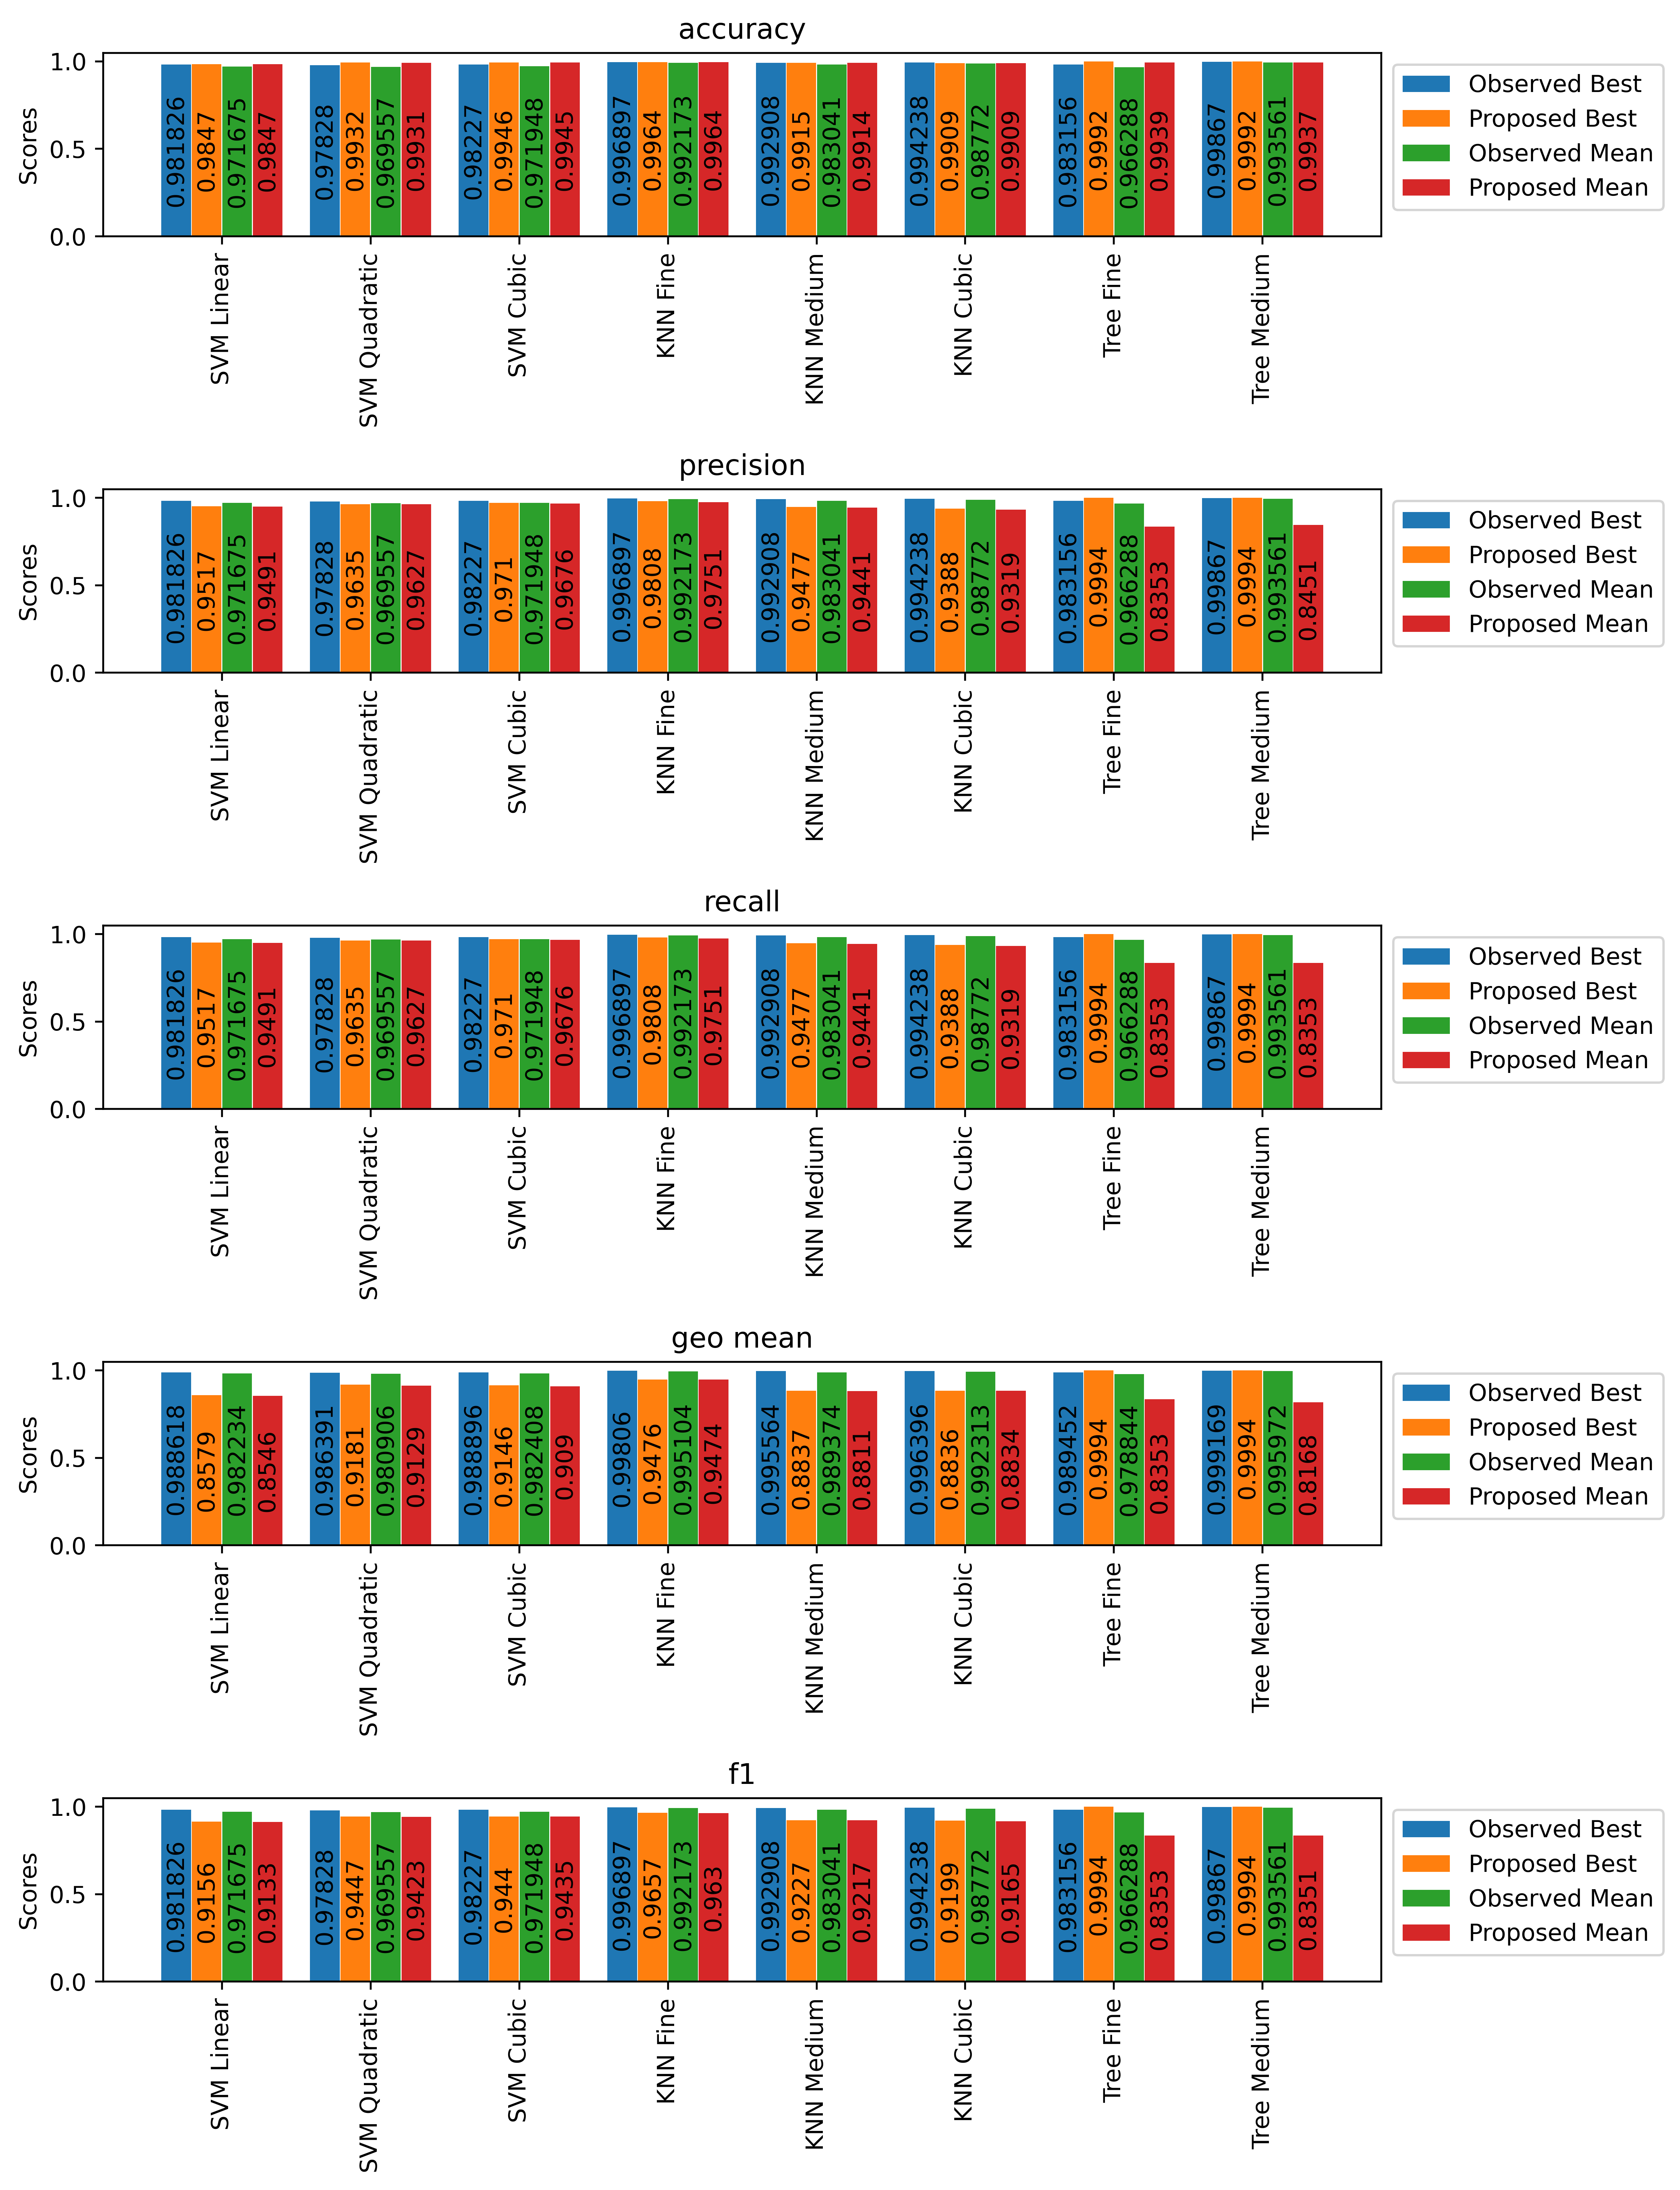
\includegraphics[width=\linewidth]{Appendices/observations.png}
    \caption{Comparison between our implementation and proposed models}
    \label{fig: comparison}
\end{figure}

\begin{table}
    \begin{tabular}{llrrrrr}
        \toprule
        model    & result & accuracy & precision & recall   & geo mean & f1       \\
        \midrule
        Voting   & best   & 0.995567 & 0.995567  & 0.995567 & 0.997228 & 0.995567 \\
                 & mean   & 0.987880 & 0.987880  & 0.987880 & 0.992413 & 0.987880 \\
                 & std    & 0.002269 & 0.002269  & 0.002269 & 0.001421 & 0.002269 \\
        AdaBoost & best   & 0.965426 & 0.965426  & 0.965426 & 0.978305 & 0.965426 \\
                 & mean   & 0.876065 & 0.876065  & 0.876065 & 0.921126 & 0.876065 \\
                 & std    & 0.050445 & 0.050445  & 0.050445 & 0.032936 & 0.050445 \\
        \bottomrule
    \end{tabular}
    \caption{The results from our solution.}
    \label{tab: our result}
\end{table}

